\documentclass{article}
\usepackage{pgfplots}
\title{KEEL: ROC output}
\begin{document}
\maketitle
\hfill \break
File: TEST
\hfill \break
\hfill \break
\begin{tikzpicture}
\begin{axis} [xlabel=False positive rate,
ylabel=True positive rate,axis x line=bottom,
axis y line=left]
\addplot coordinates { (0,0)(0,1)(1,1)};\end{axis}
\end{tikzpicture}\hfill \break
 AUC:1.0
\hfill \break
\begin{tikzpicture}
\begin{axis} [xlabel=False positive rate,
ylabel=True positive rate,axis x line=bottom,
axis y line=left]
\addplot coordinates { (0,0)(0.411764705882353,0.5454545454545455) };\end{axis}
\end{tikzpicture}\hfill \break
 AUC:0.11229946524064173
\hfill \break
\begin{tikzpicture}
\begin{axis} [xlabel=False positive rate,
ylabel=True positive rate,axis x line=bottom,
axis y line=left]
\addplot coordinates { (0,0)(0.39285714285714274,0.14285714285714285) };\end{axis}
\end{tikzpicture}\hfill \break
 AUC:0.028061224489795908
\hfill \break
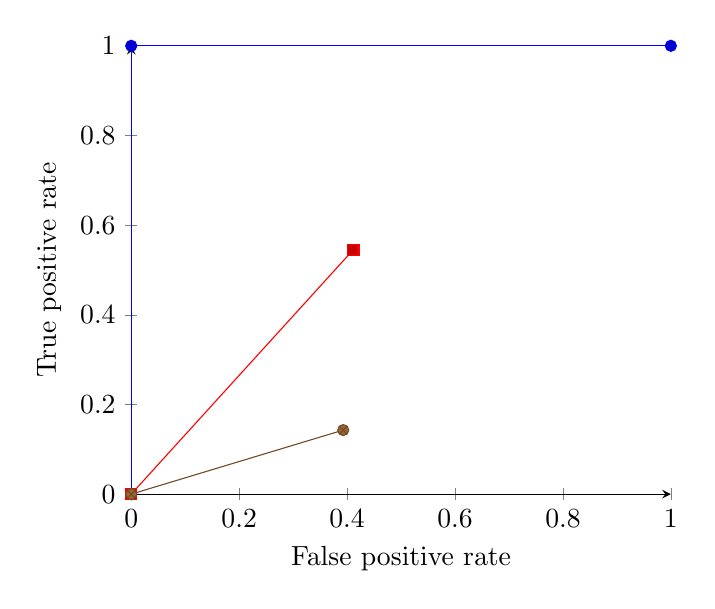
\begin{tikzpicture}
\begin{axis} [xlabel=False positive rate,
ylabel=True positive rate,axis x line=bottom,
axis y line=left]
\addplot coordinates { (0,0)(0,1)(1,1)};
\addplot coordinates { (0,0)(0.411764705882353,0.5454545454545455) };
\addplot coordinates { (0,0)(0.39285714285714274,0.14285714285714285) };
\end{axis}
\end{tikzpicture}\hfill \break
File: TRAINING
\hfill \break
\begin{tikzpicture}
\begin{axis} [xlabel=False positive rate,
ylabel=True positive rate,axis x line=bottom,
axis y line=left]
\addplot coordinates { (0,0)(0,1)(1,1)};\end{axis}
\end{tikzpicture}\hfill \break
 AUC:1.0
\hfill \break
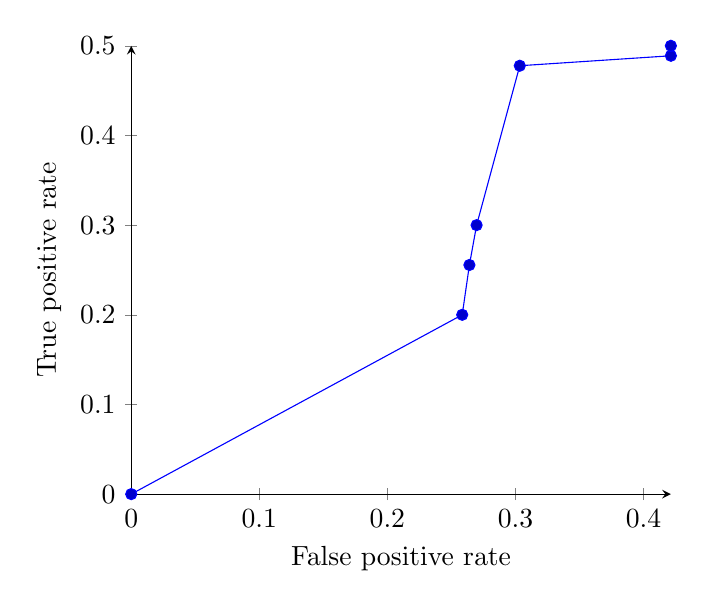
\begin{tikzpicture}
\begin{axis} [xlabel=False positive rate,
ylabel=True positive rate,axis x line=bottom,
axis y line=left]
\addplot coordinates { (0,0)(0.25842696629213513,0.19999999999999993)(0.26404494382022503,0.2555555555555554)(0.26966292134831493,0.29999999999999993)(0.30337078651685434,0.47777777777777797)(0.42134831460674227,0.4888888888888891)(0.42134831460674227,0.5000000000000002) };\end{axis}
\end{tikzpicture}\hfill \break
 AUC:0.10043695380774056
\hfill \break
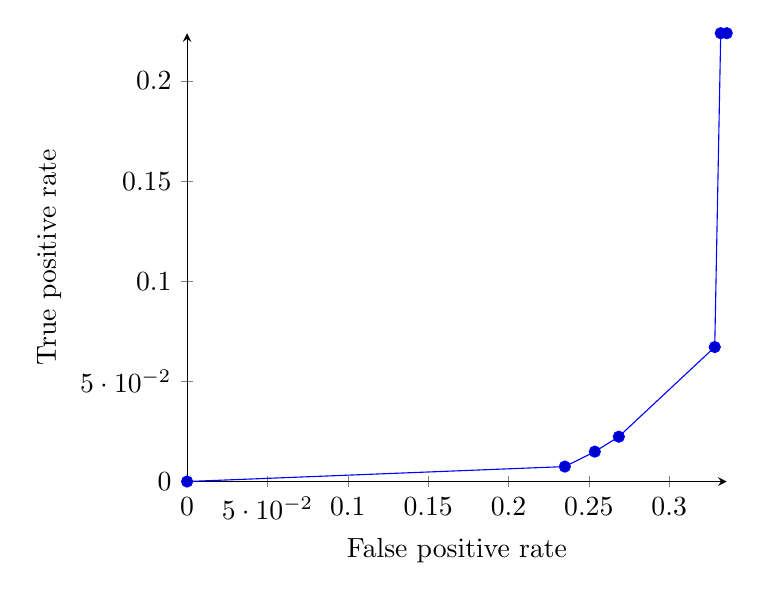
\begin{tikzpicture}
\begin{axis} [xlabel=False positive rate,
ylabel=True positive rate,axis x line=bottom,
axis y line=left]
\addplot coordinates { (0,0)(0.23507462686567188,0.007462686567164179)(0.2537313432835824,0.014925373134328358)(0.2686567164179108,0.022388059701492536)(0.3283582089552244,0.06716417910447761)(0.3320895522388065,0.22388059701492524)(0.3358208955223886,0.22388059701492524) };\end{axis}
\end{tikzpicture}\hfill \break
 AUC:0.006460236132769009
\hfill \break
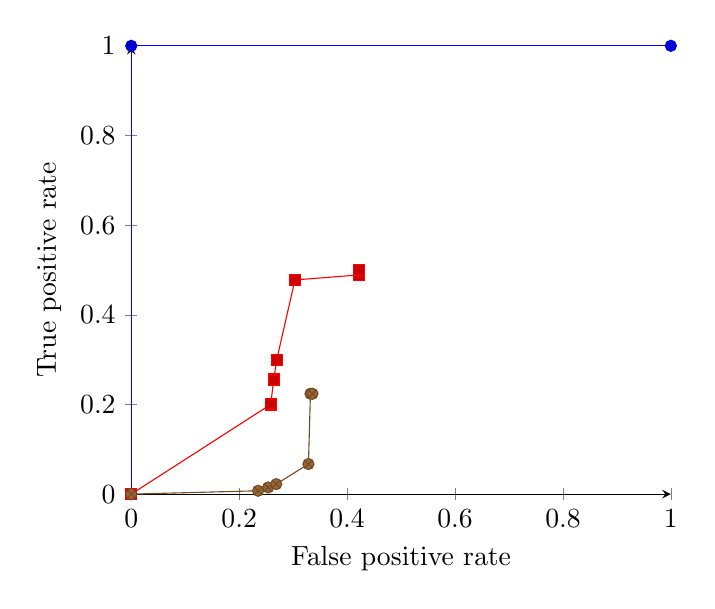
\begin{tikzpicture}
\begin{axis} [xlabel=False positive rate,
ylabel=True positive rate,axis x line=bottom,
axis y line=left]
\addplot coordinates { (0,0)(0,1)(1,1)};
\addplot coordinates { (0,0)(0.25842696629213513,0.19999999999999993)(0.26404494382022503,0.2555555555555554)(0.26966292134831493,0.29999999999999993)(0.30337078651685434,0.47777777777777797)(0.42134831460674227,0.4888888888888891)(0.42134831460674227,0.5000000000000002) };
\addplot coordinates { (0,0)(0.23507462686567188,0.007462686567164179)(0.2537313432835824,0.014925373134328358)(0.2686567164179108,0.022388059701492536)(0.3283582089552244,0.06716417910447761)(0.3320895522388065,0.22388059701492524)(0.3358208955223886,0.22388059701492524) };
\end{axis}
\end{tikzpicture}\end{document}